%!TEX root = ../localgov_GL_jpube.tex

\subsection*{Data Appendix}
\label{sec:dataappendix}

The main sample for the analysis in this paper comprises cross-sectional data about state and local governments for the 50 US States. We combine data from several sources on fiscal, employment, and demographic information at state and local levels. 

As described in Section~\ref{sec:data}, we use the Annaul Surveys of State and Local Government Finances from the Census of Governments to measure the fraction of revenues of state and local governments coming from different sources.\footnote{As of August 14, 2020, documentation for the ASSLGF is available here: https://www.census.gov/programs-surveys/gov-finances.html. An archive of the data and documentation is available from the authors upon request.} The ASSLGF files provide detailed estimates of expenditure and revenue for governments at the state and local levels, aggregated by state, from 1967 to 2017. These estimates are based on surveys of state and local governments that occur with differing frequencies and sampling rates depending on the level of government (state, county, city and township, etc.). For years ending in 2 and 7 the survey is comprehensive, for other years annual numbers are imputed from selective sampling. We use the 2017 data to create measures of state and local government exposure to different revenue sources for the regression analysis	. \emph{Sales Tax Exposure} is defined as the ratio of revenue from Sales and Gross Receipts to total Total Revenue. \emph{Income Tax Exposure} combines personal and corporate income taxes. \emph{Intergov Exposure} is defined as the revenue received from higher levels of government (federal government for states, and federal and state for local governments) as a share of total revenues. When we combine state and local governments into a single measure, intergovernmental revenues from the state are netted out. 

We measure employment using the Bureau of Labor Statistics' Current Population Survey (CPS) public use microdata. The data is retrieved from the IPUMS CPS archive at cps.ipums.org. We use the Basic Monthly samples from January to August 2020. All microdata is aggregated using the Final Basic Weights (\emph{wtfinl}) by state, month, worker class (private, federal government, state government, local government to estimate labor force characteristics of each cell. Specifically, we measure the size of the labor force, the number of people employed, number unemployed, and the number who indicate they are laid off. At this level of granularity the number of survey respondents in each cell can be small, and thus the estimates of population levels, and month to month changes in levels can be noisy. To reduce the impact of measurement error we instead focus on ratios. Specifically, we compute the estimated \emph{fraction} of workers who are laid off as the estimated number of workers laid off in a cell divided by the estimated size of the labor force in that cell. Our main variable of interest, $\Delta$\emph{Muni Laid Off}, is the change from February 2020 in the fraction of state and local government workers in a cell classified as laid off. We also compute the change from February in the more standard unemployment rate (employed divided by employed plus unemployed). For most specifications we use respondents of all occupations. We also study employment of healthcare workers specifically, which corresponds to CPS 2020 Occupation codes 3000 through 3655.  We also proxy for the tourism industry share of employment in a state by looking at the fraction of private sector workers classified with CPS 2020 Industry code 8660, ``Traveler accommodation.''








%%%%%%%%%%%%%%%%%%%%%%%%%%%%%%%%%%%%%%%%%%%%%%%%%%%%%%%%%%%%%%%%%%%%%%
\subsection*{Effect of Tax Decrease on Public Employment}
\label{subsec:empirics:generalemp}

While the events unfolding in the Spring of 2020 are remarkable, the response of states to a loss in revenue is not (see \cite{Poterba:1994:FiscalCrises}). 
We extend our analysis of the impact from local government finances to local public employment to the period spanning 1992 to 2018.
Expanding the sample sheds light on how specific the Spring 2020 moment is, as we compare the magnitudes of our estimates. 
Moreover we find that the effect of a loss of tax revenues to employment is persistent, suggesting a long-lasting impact of the COVID-19 crisis on local governments. 

To analyze state and local governments in the long run, we link both the financial files (ASSGF) and the payroll files (ASPEP) from the Census of Governments. 
In Table~\ref{table:layoffRainyDayPanel} we consider the effect of tax revenues on state and local governments employment. 
In column 1, we find that local private employment correlates positively with state and local tax revenues combined; a loss in revenue of 10\% corresponds to a decrease of 1\% in private employment, confirming the procyclical nature of local tax revenues.
In columns 2, 3, and 5, we examine separately the effect of a local change in tax revenues on local employment---for both state and local first, then state only, and finally for local governments only. 
We find a negative effect of tax revenues on unemployment, echoing the results documented above for the Spring of 2020 in Tables~\ref{table:muniLaidoffCovidDiff} and~\ref{table:muniLaidoffRobustness}. 
A 10\% decline in local tax receipts correlates with a 1.4\% decrease in local government employment, and a 10\% decline in states' tax receipts correlates with a 0.8\% decline in state employment. 

In column four, we focus on state governments to investigate the role of balanced budget requirements, and the ability of governments to implement counter-cyclical fiscal policy.
As described in Section~\ref{subsec:RainyDayFunds} and in Table~\ref{table:layoffRainyDay}, we examine the role of rainy day funds in the larger sample.
We form terciles at the state level for the level of rainy day funds as a fraction of total expenditures; we find that for states with low levels of savings the elasticity of state employment to tax revenues is 15\% larger than for states with sufficient savings (in the highest tercile). 
This result highlights the role played by the institutional rules imposing balanced budget for state governments, and highlights how constrained states have more cyclical public employment. 

Last we go beyond the contemporaneous cross-sectional relations to evaluate the persistence of the effect of tax revenues on employment. 
In Table~\ref{table:layoffPersistence}, we show how the effect of state and local government tax revenues on employment persist up to three years, suggesting that tax revenues play a role on public employment beyond their contemporaneous impact. 



%%%%%%%%%%%%%%%%%%%%%%%%%%%%%%%%%%%%%%%%%%%%%%%%%%%%%%%%%%%%%%%%%%%%%%%%%%%%%%%%%%%%%%%%%%%%%%%%%%%%%%%%%%%%%%%%%%%%%%%%%%%%%%%%%%%%%%%%%%%%%%%%%%%%%%%%%%%%%%%%%%%%%%%%%%%%%%%%%%%%%%%%%%%%%%%%%%%%%%%%%%%%%%%%%%
% APPENDIX FIGURES
%%%%%%%%%%%%%%%%%%%%%%%%%%%%%%%%%%%%%%%%%%%%%%%%%%%%%%%%%%%%%%%%%%%%%%%%%%%%%%%%%%%%%%%%%%%%%%%%%%%%%%%%%%%%%%%%%%%%%%%%%%%%%%%%%%%%%%%%%%%%%%%%%%%%%%%%%%%%%%%%%%%%%%%%%%%%%%%%%%%%%%%%%%%%%%%%%%%%%%%%%%%%%%%%%%
\clearpage

\subsection*{Appendix Figures and Tables}

\clearpage



%%%%%%%%%%%%%%%%%%%%%%%%%%%%%%%%%%%%%%%%%%%%%%%%%%%%%%%%%%%%%%%%
%% SCATTERPLOT OF MAIN SHORT RUN RESULT
\begin{center}
\begin{figure}[!ht]
	\centering
	\caption{\\ Local Government Unemployment: April 2020 \\
	{\small Figure~\ref{figure:unconditionalScatterSalesShare} shows the relationship between state and local governments' \emph{Sales Tax Dependence} and the unemployment rate of state and local government workers in that state in April 2020. \emph{Sales Tax Dependence} is defined as the fraction of state and local government revenues derived from sales taxes. The April 2020 unemployment rate among state and local government workers in a state is measured from the April 2020 CPS Survey as the (sampling weighted) fraction of respondents working for state and local governments in a state indicating they had been laid off.}}
	\label{figure:unconditionalScatterSalesShare}
	\includegraphics[scale=0.9]{../output/appendix/figures/muni_laidofffrac_salestax_april2020.eps}
\end{figure}
\end{center}

%%%%%%%%%%%%%%%%%%%%%%%%%%%%%%%%%%%%%%%%%%%%%%%%%%%%%%%%%%%%%%%%


%%%%%%%%%%%%%%%%%%%%%%%%%%%%%%%%%%%%%%%%%%%%%%%%%%%%%%%%%%%%%%%%
%% CARES ACT POPULATION

\begin{center}
\begin{figure}[!ht]
	\centering
	\caption{\\ CARES Funding and State Population. \\
	{\small Figure~\ref{figure:cares_formula} plots the CARES Act funding received by a state against state population, as measured from 2019 Census estimates. Small states received identical awards of \$1.25 billion, and larger states received funding proportional to their population.}}
	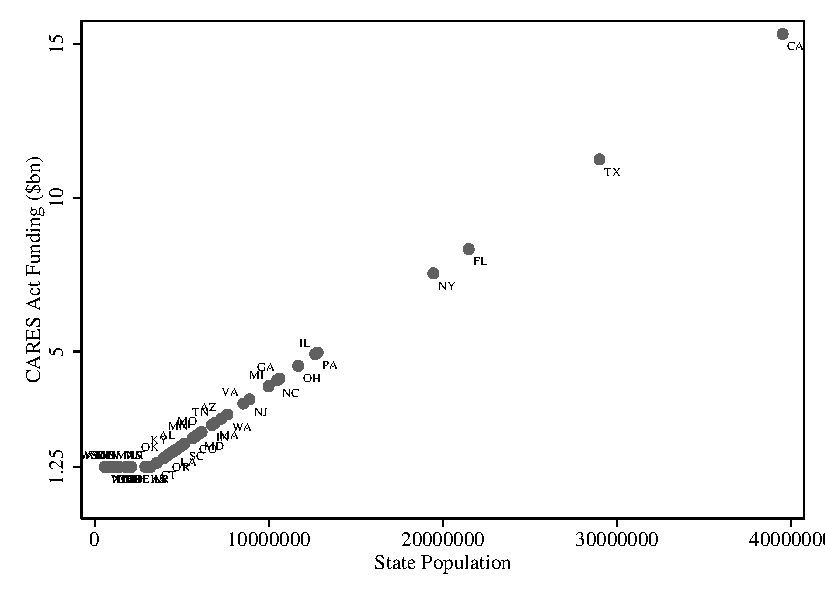
\includegraphics[scale=1.1]{../output/appendix/figures/cares_formula.pdf}
	
	\label{figure:cares_formula}
\end{figure}
\end{center}

%%%%%%%%%%%%%%%%%%%%%%%%%%%%%%%%%%%%%%%%%%%%%%%%%%%%%%%%%%%%%%%%


%%%%%%%%%%%%%%%%%%%%%%%%%%%%%%%%%%%%%%%%%%%%%%%%%%%%%%%%%%%%%%%%%%%%%%%%%%%%%%%%%%%%%%%%%%%%%%%%%%%%%%%%%%%%%%%%%%%%%%%%%%%%%%%%%%%%%%%%%%%%%%%%%%%%%%%%%%%%%%%%%%%%%%%%%%%%%%%%%%%%%%%%%%%%%%%%%%%%%%%%%%%%%%%%%%
% APPENDIX TABLES
%%%%%%%%%%%%%%%%%%%%%%%%%%%%%%%%%%%%%%%%%%%%%%%%%%%%%%%%%%%%%%%%%%%%%%%%%%%%%%%%%%%%%%%%%%%%%%%%%%%%%%%%%%%%%%%%%%%%%%%%%%%%%%%%%%%%%%%%%%%%%%%%%%%%%%%%%%%%%%%%%%%%%%%%%%%%%%%%%%%%%%%%%%%%%%%%%%%%%%%%%%%%%%%%%%

\clearpage

%%%%%%%%%%%%%%%%%%%%%%%%%%%%%%%%%%%%%%%%%%%%%%%%%%%%%%%%%%%%%%%%%%%%%%%%%%%%%%%%%%%%%%%%%%%%%%%%%%%%%%%%%
% \pagestyle{empty}
\begin{table} %[!ht]
\begin{center}
\begin{threeparttable}

\caption{\\ Breakdown of State and Local Government Employment Declines}
\label{table:summary_occupation}

\centering 

\begin{small}

  


%\begin{table}[hbt]
%\begin{threeparttable}[b]
%\caption{Asset Pricing: Portfolios Sorted on both Elasticities: $\zeta_h$ and $\eta_h$}
%\label{table:elasticty-all-1}
%\begin{small}
% \setlength{\tabcolsep}{0.5\tabcolsep}
%{\textwidth}

 % \begin{tabular*}{1\textwidth}{@{}l@{\extracolsep{\fill}} YYY @{}} 
\begin{tabular*}{0.85\textwidth}{@{}l YYY @{ }} 


\cmidrule[1.0pt](l{-1em} r{-1em}){1-4} 
\addlinespace

% \cmidrule[1pt](l{0.5em} r{0.5em}){2-4} 
%  & \multicolumn{3}{c}{Panel A: Summary Statistics across Elasticity Groups, $\zeta$} \\
% \cmidrule[0.5pt](l{0.5em} r{0.5em}){2-4} 



%%%%%%%%%%%%%%%%%%%%%%%%%%%%%%%%%%%%%%%%%%%%%%%%%%%%%%%%%%%%%%%%%%%%%%%%%%%%%%%%%%%


\multicolumn{1}{c}{} & 
\multicolumn{3}{c}{Panel A. State Governments Employment by Occupations} \\

\cmidrule[0.5pt](l{0.5em} r{0.5em}){2-4}


% Set up the first
& 
   \multicolumn{1}{c}{Employment by Occupation} & 
   \multicolumn{1}{c}{Change in Employment} & 
   \multicolumn{1}{c}{Fraction of Total Layoffs} \\

& 
   \multicolumn{1}{c}{(pct. in Feb.)} & 
   \multicolumn{1}{c}{(in pct. from Feb. to Apr.)} & 
   \multicolumn{1}{c}{(in pct. of total change)} 
   \\

\cmidrule[0.5pt](l{0.5em} r{0.5em}){2-2}
\cmidrule[0.5pt](l{0.5em} r{0.5em}){3-3}
\cmidrule[0.5pt](l{0.5em} r{0.5em}){4-4}


%%%%%%%%%%%%%%%%%%%%%%%%%%%%%%%%%%%%%%%%%%%%%%%%%%%%%%%%%%%%%%%%%%%%%%%%%%%%%%%%%%%
\multicolumn{1}{l}{Education} &
30.4 &
-11.2 &
40.2 \\

\multicolumn{1}{l}{Administrative}  &
10.7 &
-11.8 &
15 \\

\multicolumn{1}{l}{Healthcare} & 
9.78 &
-3.74 &
4.34 \\

\multicolumn{1}{l}{Protective Services} & 
6.98 &
0.9 &
-0.75 \\

\multicolumn{1}{l}{Management} & 
6.62 &
-6.44 &
5.05 \\

\multicolumn{1}{l}{Other} & 
35.5 &
-8.59 &
36.2 \\
%%%%%%%%%%%%%%%%%%%%%%%%%%%%%%%%%%%%%%%%%%%%%%%%%%%%%%%%%%%%%%%%%%%%%%%%%%%%%



%%%%%%%%%%%%%%%%%%%%%%%%%%%%%%%%%%%%%%%%%%%%%%%%%%%%%%%%%%%%%%%%%%%%%%%%%%%%%
\cmidrule[0.5pt](l{0.5em} r{0.5em}){2-4}

\multicolumn{1}{c}{} & 
\multicolumn{3}{c}{Panel B. Local Governments} \\

\cmidrule[0.5pt](l{0.5em} r{0.5em}){2-4}
%%%%%%%%%%%%%%%%%%%%%%%%%%%%%%%%%%%%%%%%%%%%%%%%%%%%%%%%%%%%%%%%%%%%%%%%%%%%%



%%%%%%%%%%%%%%%%%%%%%%%%%%%%%%%%%%%%%%%%%%%%%%%%%%%%%%%%%%%%%%%%%%%%%%%%%%%%%%%%%%%
\multicolumn{1}{l}{Education} & 
33.4 &
-18.5 &
34.2 \\

\multicolumn{1}{l}{Administrative} & 
10.5 &
-19.5 &
11.4 \\

\multicolumn{1}{l}{Healthcare} & 
5.9 &
-21.3 &
6.95 \\

\multicolumn{1}{l}{Protective Services} & 
12.8 &
-15.7 &
11.1 \\

\multicolumn{1}{l}{Management} & 
4.58 &
1.07 &
-0.27 \\

\multicolumn{1}{l}{Other} & 
32.8 &
-20.2 &
36.7 \\
%%%%%%%%%%%%%%%%%%%%%%%%%%%%%%%%%%%%%%%%%%%%%%%%%%%%%%%%%%%%%%%%%%%%%%%%%%%%%




           
\cmidrule[1.5pt](l{-1em} r{-1em}){1-4} 


\end{tabular*}


\end{small}

\begin{footnotesize}
\begin{tablenotes}
\item The table reports occupation-level aggregate summary statistics for state and local government employment in February 2020 and declines through April 2020 from the \emph{Current Population Survey}. Panels A and B report statistics on employment at state and local levels of government, respectively. The first column shows the breakdown of total government employees in the United States by broad categories of occupation. The second column shows the percent change in number of workers in each occupation from February to April 2020 as estimated from the CPS data. The final column reports the share of total declines in employment over this period stemming from each industry.    
\end{tablenotes}
\end{footnotesize}
\end{threeparttable}
\end{center}
\end{table}
\thispagestyle{empty}
%%%%%%%%%%%%%%%%%%%%%%%%%%%%%%%%%%%%%%%%%%%%%%%%%%%%%%%%%%%%%%%%%%%%%%%%%%%%%%%%%%%%%%%%%%%%%%%%%%%%%%%%%%%%%%%%


%%%%%%%%%%%%%%%%%%%%%%%%%%%%%%%%%%%%%%%%%%%%%%%%%%%%%%%%%%%%%%%%%%%%%%%%%%%%%%%%%%%%%%%%%%%%%%%%%%%%%%%%%
% \pagestyle{empty}
\begin{table} %[!ht]
\begin{center}
\begin{threeparttable}

\caption{\\ Tax Revenues by Population across States}
\label{table:taxrev2}

\centering 

\begin{small}

  


%\begin{table}[hbt]
%\begin{threeparttable}[b]
%\caption{Asset Pricing: Portfolios Sorted on both Elasticities: $\zeta_h$ and $\eta_h$}
%\label{table:elasticty-all-1}
%\begin{small}
% \setlength{\tabcolsep}{0.5\tabcolsep}
%{\textwidth}

 % \begin{tabular*}{1\textwidth}{@{}l@{\extracolsep{\fill}} YYYYY @{}} 
\begin{tabular*}{0.85\textwidth}{@{}l YYYYY @{ }} 


\cmidrule[1.0pt](l{-1em} r{-1em}){1-6} 
\addlinespace

% \cmidrule[1pt](l{0.5em} r{0.5em}){2-6} 
%  & \multicolumn{5}{c}{Panel A: Summary Statistics across Elasticity Groups, $\zeta$} \\
% \cmidrule[0.5pt](l{0.5em} r{0.5em}){2-6} 



%%%%%%%%%%%%%%%%%%%%%%%%%%%%%%%%%%%%%%%%%%%%%%%%%%%%%%%%%%%%%%%%%%%%%%%%%%%%%%%%%%%


\multicolumn{1}{c}{} & 
\multicolumn{5}{c}{Panel A. State Governments} \\

\cmidrule[0.5pt](l{0.5em} r{0.5em}){2-6}


% Set up the first
& 
   \multicolumn{1}{c}{Average} & 
   \multicolumn{1}{c}{Min} & 
   \multicolumn{1}{c}{25th pct.} & 
   \multicolumn{1}{c}{75th pct.} & 
   \multicolumn{1}{c}{Max} \\

\cmidrule[0.5pt](l{0.5em} r{0.5em}){2-2}
\cmidrule[0.5pt](l{0.5em} r{0.5em}){3-3}
\cmidrule[0.5pt](l{0.5em} r{0.5em}){4-4}
\cmidrule[0.5pt](l{0.5em} r{0.5em}){5-5}
\cmidrule[0.5pt](l{0.5em} r{0.5em}){6-6}


%%%%%%%%%%%%%%%%%%%%%%%%%%%%%%%%%%%%%%%%%%%%%%%%%%%%%%%%%%%%%%%%%%%%%%%%%%%%%%%%%%%


\multicolumn{1}{l}{Total Tax Revenues} & 
\multicolumn{5}{c}{} \\

\multicolumn{1}{l}{\quad $\sigma(\Delta\text{tax})$} & 
0.084 &
0.034 &
0.068 &
0.092 &
0.199 
\\

\addlinespace

\multicolumn{1}{l}{Sales Tax} & 
\multicolumn{5}{c}{} \\

\multicolumn{1}{l}{\quad $\sigma(\Delta\text{tax})$} & 
0.06 &
0.028 &
0.045 &
0.071 &
0.14 
\\

\multicolumn{1}{l}{\quad Share of total rev.} & 
0.252 &
0 &
0.192 &
0.283 &
0.597 
\\

% \addlinespace

\multicolumn{1}{l}{Indiv. Income Tax} & 
\multicolumn{5}{c}{} \\

\multicolumn{1}{l}{\quad $\sigma(\Delta\text{tax})$} & 
0.087 &
0.045 &
0.065 &
0.094 &
0.229 
\\

\multicolumn{1}{l}{\quad Share of total rev.} & 
0.219 &
0 &
0.185 &
0.294 &
0.434 
\\

% \addlinespace

\multicolumn{1}{l}{Corp. Income Tax} & 
\multicolumn{5}{c}{} \\

\multicolumn{1}{l}{\quad $\sigma(\Delta\text{tax})$} & 
0.103 &
0.053 &
0.074 &
0.113 &
0.289 
\\

\multicolumn{1}{l}{\quad Share of total rev.} & 
0.248 &
0 &
0.215 &
0.3 &
0.423 
\\

\addlinespace



%%%%%%%%%%%%%%%%%%%%%%%%%%%%%%%%%%%%%%%%%%%%%%%%%%%%%%%%%%%%%%%%%%%%%%%%%%%%%
\cmidrule[0.5pt](l{0.5em} r{0.5em}){2-6}

\multicolumn{1}{c}{} & 
\multicolumn{5}{c}{Panel B. Local Governments} \\

\cmidrule[0.5pt](l{0.5em} r{0.5em}){2-6}
%%%%%%%%%%%%%%%%%%%%%%%%%%%%%%%%%%%%%%%%%%%%%%%%%%%%%%%%%%%%%%%%%%%%%%%%%%%%%



\multicolumn{1}{l}{Total Tax Revenues} & 
\multicolumn{5}{c}{} \\

\multicolumn{1}{l}{\quad $\sigma(\Delta\text{tax})$} & 
0.202 &
0.056 &
0.131 &
0.24 &
0.561 
\\

\addlinespace

\multicolumn{1}{l}{Property Tax} & 
\multicolumn{5}{c}{} \\

\multicolumn{1}{l}{\quad $\sigma(\Delta\text{tax})$} & 
0.203 &
0.067 &
0.127 &
0.251 &
0.546 
\\

\multicolumn{1}{l}{\quad Share of total rev.} & 
0.634 &
0.215 &
0.452 &
0.849 &
0.983 
\\

% \addlinespace

\multicolumn{1}{l}{Sales Tax} & 
\multicolumn{5}{c}{} \\

\multicolumn{1}{l}{\quad $\sigma(\Delta\text{tax})$} & 
0.237 &
0.037 &
0.126 &
0.265 &
0.991 
\\

\multicolumn{1}{l}{\quad Share of total rev.} & 
0.16 &
0 &
0 &
0.269 &
0.641 
\\

\addlinespace



%%%%%%%%%%%%%%%%%%%%%%%%%%%%%%%%%%%%%%%%%%%%%%%%%%%%%%%%%%%%%%%%%%%%%%%%%%%%%
\cmidrule[0.5pt](l{0.5em} r{0.5em}){2-6}

\multicolumn{1}{c}{} & 
\multicolumn{5}{c}{Panel C. State \& Local Governments} \\

\cmidrule[0.5pt](l{0.5em} r{0.5em}){2-6}
%%%%%%%%%%%%%%%%%%%%%%%%%%%%%%%%%%%%%%%%%%%%%%%%%%%%%%%%%%%%%%%%%%%%%%%%%%%%%



\multicolumn{1}{l}{Total Tax Revenues} & 
\multicolumn{5}{c}{} \\

\multicolumn{1}{l}{\quad $\sigma(\Delta\text{tax})$} & 
0.071 &
0.044 &
0.062 &
0.075 &
0.135 
\\

\addlinespace

\multicolumn{1}{l}{Property Tax} & 
\multicolumn{5}{c}{} \\

\multicolumn{1}{l}{\quad $\sigma(\Delta\text{tax})$} & 
0.144 &
0.051 &
0.093 &
0.16 &
0.423 
\\

\multicolumn{1}{l}{\quad Share of total rev.} & 
0.264 &
0.115 &
0.217 &
0.302 &
0.568 
\\

% \addlinespace

\multicolumn{1}{l}{Sales Tax} & 
\multicolumn{5}{c}{} \\

\multicolumn{1}{l}{\quad $\sigma(\Delta\text{tax})$} & 
0.066 &
0.028 &
0.049 &
0.074 &
0.188 
\\

\multicolumn{1}{l}{\quad Share of total rev.} & 
0.215 &
0 &
0.162 &
0.259 &
0.485 
\\


% \addlinespace

\multicolumn{1}{l}{Indiv. Income Tax} & 
\multicolumn{5}{c}{} \\

\multicolumn{1}{l}{\quad $\sigma(\Delta\text{tax})$} & 
0.086 &
0.045 &
0.065 &
0.094 &
0.221 
\\

\multicolumn{1}{l}{\quad Share of total rev.} & 
0.179 &
0 &
0.143 &
0.242 &
0.335 
\\

% \addlinespace

\multicolumn{1}{l}{Corp. Income Tax} & 
\multicolumn{5}{c}{} \\

\multicolumn{1}{l}{\quad $\sigma(\Delta\text{tax})$} & 
0.101 &
0.051 &
0.076 &
0.108 &
0.261 
\\

\multicolumn{1}{l}{\quad Share of total rev.} & 
0.188 &
0 &
0.156 &
0.236 &
0.301 
\\

           
\cmidrule[1.5pt](l{-1em} r{-1em}){1-6} 


\end{tabular*}


\end{small}

\begin{footnotesize}
\begin{tablenotes}
\item The table reports summary statistics of tax revenues per capita for State and Local governments from 1980 to 2017. Panel A reports estimates for State governments. $\sigma(\Delta\text{tax})$ is the standard deviation of the year-on-year growth of taxes by categories across states. Estimates report the average, minimum, maximum, 25th and 75th percentile of the volatility of taxes across states and the same statistics of the average share of tax categories in total taxes. Panel B reports estimates for local governments (county, municipal and township governments). Statistics are the same as in Panel B. Panel C reports the same statistics for state and local government aggregated at the state level from the Census of Governments ASSLGF files.
\end{tablenotes}
\end{footnotesize}
\end{threeparttable}
\end{center}
\end{table}
\thispagestyle{empty}
%%%%%%%%%%%%%%%%%%%%%%%%%%%%%%%%%%%%%%%%%%%%%%%%%%%%%%%%%%%%%%%%%%%%%%%%%%%%%%%%%%%%%%%%%%%%%%%%%%%%%%%%%%%%%%%%




%%%%%%%%%%%%%%%%%%%%%%%%%%%%%%%%%%%%%%%%%%%%%%%%%%%%%%%%%%%%%%%%%%%%%%%%%%%%%%%%%%%%%%%%%%%%%%%%%%%%%%%%%
% \pagestyle{empty}
\begin{landscape}

\begin{table}[!ht]
\begin{center}
\begin{threeparttable}

\caption{\\ National Unemployment during the COVID-19 Crisis}
\label{table:unemp:national1}

\centering 

\begin{small}

  

 \setlength\sparkbottomlinethickness{.2pt}

%\begin{table}[hbt]
%\begin{threeparttable}[b]
%\caption{Asset Pricing: Portfolios Sorted on both Elasticities: $\zeta_h$ and $\eta_h$}
%\label{table:elasticty-all-1}
%\begin{small}
% \setlength{\tabcolsep}{0.5\tabcolsep}
%{\textwidth}

 % \begin{tabular*}{1\textwidth}{@{}l@{\extracolsep{\fill}} YYYYYYY @{}} 
\begin{tabular*}{0.85\textwidth}{@{}l YYYYYYY @{ }} 


\cmidrule[1.5pt](l{-1em} r{-1em}){1-8} 
\addlinespace

% \cmidrule[1pt](l{0.5em} r{0.5em}){2-8} 
%  & \multicolumn{7}{c}{Panel A: Summary Statistics across Elasticity Groups, $\zeta$} \\
% \cmidrule[0.5pt](l{0.5em} r{0.5em}){2-8} 



%%%%%%%%%%%%%%%%%%%%%%%%%%%%%%%%%%%%%%%%%%%%%%%%%%%%%%%%%%%%%%%%%%%%%%%%%%%%%%%%%%%





% Set up the first
& 
   \multicolumn{1}{c}{Feb.} & 
   \multicolumn{1}{c}{Mar.} & 
   \multicolumn{1}{c}{Apr.} & 
   \multicolumn{1}{c}{May.} & 
   \multicolumn{1}{c}{June.} & 
   \multicolumn{2}{c}{}  
   \\


\cmidrule[0.5pt](l{0.5em} r{0.5em}){2-8}


%%%%%%%%%%%%%%%%%%%%%%%%%%%%%%%%%%%%%%%%%%%%%%%%%%%%%%%%%%%%%%%%%%%%%%%%%%%%%%%%%%%


\multicolumn{1}{l}{Private Sector Unemployment} & 
\multicolumn{6}{c}{} \\

\multicolumn{1}{l}{\quad (in thousands of workers)} & 
4,939 &
5,886 &
18,279 &
16,647 &
13,824 &
\multicolumn{2}{c}{
	\begin{sparkline}{10}
\spark 0 0 0.166666666666667 0.0709911165989078 0.333333333333333 1 0.5 0.877687172323542 0.666666666666667 0.666037825739482 0.833333333333333 0.579168116509284 1 0.412087772244459 /
\sparkdot 1 0.412087772244459 red 
\sparkbottomline[1]
\end{sparkline} 
}
\\

\multicolumn{1}{l}{\quad (unemployment rate in \%)} & 
4.38 &
5.35 &
18 &
15.9 &
12.8 &
\multicolumn{2}{c}{}	
\\


% \addlinespace

\multicolumn{1}{l}{State Government Unemployment} & 
\multicolumn{4}{c}{} \\

\multicolumn{1}{l}{\quad (in thousands of workers)} & 
78.1 &
172 &
624 &
474 & 
501 & 
\multicolumn{2}{c}{
	\begin{sparkline}{10}
\spark 0 0 0.166666666666667 0.171260788822108 0.333333333333333 1 0.5 0.725656259468054 0.666666666666667 0.774142490243412 0.833333333333333 0.830867757230022 1 0.584230475186031 /
\sparkdot 1 0.584230475186031 red 
\sparkbottomline[1]
\end{sparkline} 
}

\\

\multicolumn{1}{l}{\quad (unemployment rate in \%)} & 
1.09 &
2.49 &
8.78 &
6.69 &
7.35 &
\multicolumn{2}{c}{}	
\\

% \addlinespace

\multicolumn{1}{l}{Local Government Unemployment} & 
\multicolumn{4}{c}{} \\

\multicolumn{1}{l}{\quad (in thousands of workers)} & 
131 &
245 &
1,201 &
931 &
881 &
\multicolumn{2}{c}{
	\begin{sparkline}{10}
\spark 0 0 0.166666666666667 0.10613147225403 0.333333333333333 1 0.5 0.747979360565313 0.666666666666667 0.701209688983054 0.833333333333333 0.86975658915184 1 0.52193071053605 /
\sparkdot 1 0.52193071053605 red 
\sparkbottomline[1]
\end{sparkline} 
}

\\

\multicolumn{1}{l}{\quad (unemployment rate in \%)} & 
1.27 &
2.42 &
12.6 &
9.51 &
9.83 &
\multicolumn{2}{c}{}	
\\


\multicolumn{1}{l}{Federal Government Unemployment} & 
\multicolumn{4}{c}{} \\

\multicolumn{1}{l}{\quad (in thousands of workers)} & 
135 &
78.2 &
201 &
188 &
218 &
\multicolumn{2}{c}{
	\begin{sparkline}{10}
\spark 0 0.408097076972474 0.166666666666667 0 0.333333333333333 0.880827249771595 0.5 0.786241294419372 0.666666666666667 1 0.833333333333333 0.764459148030476 1 0.277924546678064 /
\sparkdot 1 0.277924546678064 red 
\sparkbottomline[1]
\end{sparkline} 
}
\\

\multicolumn{1}{l}{\quad (unemployment rate in \%)} & 
3.64 &
2.1 &
5.75 &
4.95 &
5.55 &
\multicolumn{2}{c}{}	
\\



           
\cmidrule[1.5pt](l{-1em} r{-1em}){1-8} 


\end{tabular*}


\end{small}

\begin{footnotesize}
\begin{tablenotes}
\item  We report the level of sectoral unemployment from Current Population Survey (CPS), for the four sectors of private, state, local and federal governments. Sectoral unemployment is defined as the number of individuals who are not currently employed and whose last primary job was in a given sector. The sectoral unemployment rate is the ratio of sectoral unemployment scaled by the total number of individuals whose current or last job was in a given sector. The last column summarizes the time series of employment in each sector.
\end{tablenotes}
\end{footnotesize}
\end{threeparttable}
\end{center}
\end{table}

\thispagestyle{empty}

\end{landscape}
%%%%%%%%%%%%%%%%%%%%%%%%%%%%%%%%%%%%%%%%%%%%%%%%%%%%%%%%%%%%%%%%%%%%%%%%%%%%%%%%%%%%%%%%%%%%%%%%%%%%%%%%%%%%%%%%



%%%%%%%%%%%%%%%%%%%%%%%%%%%%%%%%%%%%%%%%%%%%%%%%%%%%%%%%%%%%%%%%%%%%%%%%%%%%%%%%%%%%%%%%%%%%%%%%%%%%%%%%%
% State and Local Separately
%%%%%%%%%%%%%%%%%%%%%%%%%%%%%%%%%%%%%%%%%%%%%%%%%%%%%%%%%%%%%%%%%%%%%%%%%%%%%%%%%%%%%%%%%%%%%%%%%%%%%%%%%
% \pagestyle{empty}
\begin{landscape}
\begin{table}[!ht]
\begin{center}
\begin{threeparttable}

\caption{\\ Short Run Unemployment Response of State and Local Governments Separately}
\label{table:muniLaidoffStateandLocal}

\centering 

\begin{small}

	{
\def\sym#1{\ifmmode^{#1}\else\(^{#1}\)\fi}
\begin{tabular}{l*{6}{D{.}{.}{-1}}}
\toprule
                    &\multicolumn{1}{c}{(1)}&\multicolumn{1}{c}{(2)}&\multicolumn{1}{c}{(3)}&\multicolumn{1}{c}{(4)}&\multicolumn{1}{c}{(5)}&\multicolumn{1}{c}{(6)}\\
                    &\multicolumn{1}{c}{$\Delta$ Muni Laid Off}&\multicolumn{1}{c}{$\Delta$ Muni Laid Off}&\multicolumn{1}{c}{$\Delta$ State Laid Off}&\multicolumn{1}{c}{$\Delta$ State Laid Off}&\multicolumn{1}{c}{$\Delta$ Local Laid Off}&\multicolumn{1}{c}{$\Delta$ Local Laid Off}\\
\midrule
Sales Tax Exposure  &        0.42\sym{***}&        0.26\sym{**} &        0.49\sym{***}&        0.36\sym{***}&        0.29\sym{*}  &        0.11         \\
                    &      (4.24)         &      (2.30)         &      (3.46)         &      (2.79)         &      (1.71)         &      (0.59)         \\
COVID Infection Rate&                     &      -0.052\sym{**} &                     &      -0.071\sym{*}  &                     &      -0.046         \\
                    &                     &     (-2.24)         &                     &     (-2.00)         &                     &     (-1.51)         \\
COVID Death Rate    &                     &        2.29\sym{**} &                     &        3.02\sym{*}  &                     &        2.19\sym{*}  \\
                    &                     &      (2.14)         &                     &      (1.74)         &                     &      (1.78)         \\
Log Population      &                     &       0.014\sym{**} &                     &      0.0050         &                     &       0.023\sym{***}\\
                    &                     &      (2.44)         &                     &      (0.71)         &                     &      (3.10)         \\
$\Delta$ Private Laid Off&                     &        0.14         &                     &        0.10         &                     &       0.051         \\
                    &                     &      (1.53)         &                     &      (0.63)         &                     &      (0.30)         \\
Constant            &       0.026\sym{*}  &       -0.18\sym{**} &   -0.000022         &      -0.071         &       0.052\sym{*}  &       -0.29\sym{***}\\
                    &      (1.70)         &     (-2.20)         &   (-0.0012)         &     (-0.74)         &      (1.98)         &     (-2.74)         \\
\midrule
N                   &          50         &          50         &          50         &          50         &          50         &          50         \\
$ R^2$              &        0.20         &        0.38         &        0.21         &        0.31         &       0.060         &        0.25         \\
\bottomrule
\multicolumn{7}{l}{\footnotesize \textit{t} statistics in parentheses}\\
\multicolumn{7}{l}{\footnotesize \sym{*} \(p<0.1\), \sym{**} \(p<0.05\), \sym{***} \(p<0.01\)}\\
\end{tabular}
}


\end{small}

\begin{footnotesize}
\begin{tablenotes}
\item This table reports robustness analysis of the relationship between public sector employment and the revenue composition of state and local governments. Columns 1 and 2 repeats the first two columns of Table~\ref{table:muniLaidoffCovidDiff}. Columns 3 and 4 reproduce the same specifications changing the dependent variable to the change in employment of \emph{state} government workers. Columns 5 and 6 use as the dependent variable the change in employment of \emph{local} government workers. In all specifications \emph{Sales Tax Exposure} is defined the same way, as the share of state \emph{and} local government revenues coming from sales taxes. All variables are defined as in Table~\ref{table:muniLaidoffCovidDiff}. $t$-statistics for heteroskedasticity-robust standard errors are reported in parenthesis. 

\end{tablenotes}
\end{footnotesize}
\end{threeparttable}
\end{center}
\end{table}
\thispagestyle{empty}
\end{landscape}
%%%%%%%%%%%%%%%%%%%%%%%%%%%%%%%%%%%%%%%%%%%%%%%%%%%%%%%%%%%%%%%%%%%%%%%%%%%%%%%%%%%%%%%%%%%%%%%%%%%%%%%%%%%%%%%%





%%%%%%%%%%%%%%%%%%%%%%%%%%%%%%%%%%%%%%%%%%%%%%%%%%%%%%%%%%%%%%%%%%%%%%%%%%%%%%%%%%%%%%%%%%%%%%%%%%%%%%%%%
% CROSS SECTIONAL LAYOFF ROBUSTNESS
%%%%%%%%%%%%%%%%%%%%%%%%%%%%%%%%%%%%%%%%%%%%%%%%%%%%%%%%%%%%%%%%%%%%%%%%%%%%%%%%%%%%%%%%%%%%%%%%%%%%%%%%%
% \pagestyle{empty}
\begin{landscape}
\begin{table}[!ht]
\begin{center}
\begin{threeparttable}

\caption{\\ Short Run Unemployment Response of State and Local Governments: Robustness}
\label{table:muniLaidoffRobustness}

\centering 

\begin{small}

	{
\def\sym#1{\ifmmode^{#1}\else\(^{#1}\)\fi}
\begin{tabular}{l*{5}{D{.}{.}{-1}}}
\toprule
                    &\multicolumn{1}{c}{(1)}&\multicolumn{1}{c}{(2)}&\multicolumn{1}{c}{(3)}&\multicolumn{1}{c}{(4)}&\multicolumn{1}{c}{(5)}\\
                    &\multicolumn{1}{c}{$\Delta$ Muni Laid Off}&\multicolumn{1}{c}{$\Delta$ Muni Laid Off}&\multicolumn{1}{c}{$\Delta$ Muni U/R}&\multicolumn{1}{c}{$\Delta$ Muni Laid Off}&\multicolumn{1}{c}{$\Delta$ Part Time}\\
\midrule
Sales Tax Exposure  &        0.28\sym{**} &        0.36\sym{**} &        0.51         &     -0.0083         &      -0.078         \\
                    &      (2.09)         &      (2.30)         &      (1.67)         &     (-0.24)         &     (-0.38)         \\
Property Tax Exposure&     -0.0041         &      0.0099         &       -0.16         &     -0.0038         &       0.042         \\
                    &    (-0.037)         &     (0.062)         &     (-0.61)         &     (-0.13)         &      (0.16)         \\
Intergov Exposure   &     -0.0014         &       0.014         &       0.014         &      -0.054         &      -0.077         \\
                    &   (-0.0079)         &     (0.073)         &     (0.039)         &     (-1.19)         &     (-0.37)         \\
Income Tax Exposure &       0.069         &        0.13         &        0.23         &      0.0047         &       -0.32\sym{*}  \\
                    &      (0.51)         &      (0.96)         &      (0.97)         &      (0.24)         &     (-1.90)         \\
COVID Infection Rate&      -0.055\sym{**} &      -0.051\sym{**} &      -0.087         &    -0.00092         &       0.024         \\
                    &     (-2.14)         &     (-2.27)         &     (-1.53)         &     (-0.17)         &      (0.73)         \\
COVID Death Rate    &        2.38\sym{**} &        2.03\sym{**} &        3.50         &       0.060         &       -1.49         \\
                    &      (2.06)         &      (2.17)         &      (1.38)         &      (0.27)         &     (-1.34)         \\
Log Population      &       0.013\sym{*}  &       0.018\sym{**} &       0.031\sym{**} &     -0.0016         &     -0.0072         \\
                    &      (1.78)         &      (2.50)         &      (2.08)         &     (-0.84)         &     (-0.73)         \\
$\Delta$ Private Laid Off&        0.13         &        0.12         &      -0.092         &       -0.50\sym{*}  &        0.38\sym{**} \\
                    &      (1.13)         &      (0.99)         &     (-0.36)         &     (-1.73)         &      (2.51)         \\
Tourism Employment  &       0.089         &       0.042         &       -0.55         &       -0.20         &       -0.74         \\
                    &      (0.13)         &     (0.054)         &     (-0.43)         &     (-1.14)         &     (-0.94)         \\
Constant            &       -0.17         &       -0.27\sym{**} &       -0.40         &       0.042         &        0.17         \\
                    &     (-1.39)         &     (-2.27)         &     (-1.63)         &      (1.16)         &      (0.97)         \\
\midrule
Date                &       April         &       April         &       April         &     January         &       April         \\
N                   &          50         &          50         &          50         &          50         &          50         \\
$ R^2$              &        0.38         &        0.43         &        0.33         &        0.19         &        0.20         \\
\bottomrule
\multicolumn{6}{l}{\footnotesize \textit{t} statistics in parentheses}\\
\multicolumn{6}{l}{\footnotesize \sym{*} \(p<0.1\), \sym{**} \(p<0.05\), \sym{***} \(p<0.01\)}\\
\end{tabular}
}


\end{small}

\begin{footnotesize}
\begin{tablenotes}
\item This table reports robustness analysis of the relationship between public sector employment and the revenue composition of state and local governments. Column 1 repeats the specification of Column 4 of Table~\ref{table:muniLaidoffCovidDiff} and adds as a control \emph{Tourism Employment}, the fraction of private sector employees in the state employed in the tourism industry as estimated in the CPS in February 2020. Column 2 replaces the dependent variable with the standard measure of the unemployment rate, the (sampling weighted) number of respondents in a geographic and sectoral category classified as unemployed relative to the total number of respondents in that category. Column 3 replaces the dependent variable with a measure of the change in workers moved from full to part time employment. Column 4 reports placebo results using as the dependent variable the change in the laid off fraction between November 2019 and January 2020. Column 5 reports placebo results using as the dependent variable the change from February to April 2020 in the laid off fraction of federal government workers in a given state. All variables are defined as in Table~\ref{table:muniLaidoffCovidDiff}. $t$-statistics for heteroskedasticity-robust standard errors are reported in parenthesis. 

\end{tablenotes}
\end{footnotesize}
\end{threeparttable}
\end{center}
\end{table}
\thispagestyle{empty}
\end{landscape}
%%%%%%%%%%%%%%%%%%%%%%%%%%%%%%%%%%%%%%%%%%%%%%%%%%%%%%%%%%%%%%%%%%%%%%%%%%%%%%%%%%%%%%%%%%%%%%%%%%%%%%%%%%%%%%%%


%%%%%%%%%%%%%%%%%%%%%%%%%%%%%%%%%%%%%%%%%%%%%%%%%%%%%%%%%%%%%%%%%%%%%%%%%%%%%%%%%%%%%%%%%%%%%%%%%%%%%%%%%
% CROSS SECTIONAL LAYOFF ROBUSTNESS
%%%%%%%%%%%%%%%%%%%%%%%%%%%%%%%%%%%%%%%%%%%%%%%%%%%%%%%%%%%%%%%%%%%%%%%%%%%%%%%%%%%%%%%%%%%%%%%%%%%%%%%%%
% \pagestyle{empty}
\begin{table}[!ht]
\begin{center}
\begin{threeparttable}

\caption{\\ Evolution of Local Government Unemployment Elasticities}
\label{table:mediumrun}

\centering 

\begin{small}

	{
\def\sym#1{\ifmmode^{#1}\else\(^{#1}\)\fi}
\begin{tabular}{l*{3}{c}}
\hline\hline
                    &\multicolumn{1}{c}{(1)}&\multicolumn{1}{c}{(2)}&\multicolumn{1}{c}{(3)}\\
                    &\multicolumn{1}{c}{$\Delta$ Muni Laid Off}&\multicolumn{1}{c}{$\Delta$ Muni Laid Off}&\multicolumn{1}{c}{$\Delta$ State Laid Off}\\
\hline
April $\times$ Sales Tax Exposure&       0.289\sym{**} &                     &                     \\
                    &      (2.49)         &                     &                     \\
[1em]
May $\times$ Sales Tax Exposure&       0.258\sym{*}  &                     &                     \\
                    &      (1.76)         &                     &                     \\
[1em]
June $\times$ Sales Tax Exposure&       0.210\sym{*}  &                     &                     \\
                    &      (1.79)         &                     &                     \\
[1em]
July $\times$ Sales Tax Exposure&       0.170         &                     &                     \\
                    &      (1.57)         &                     &                     \\
[1em]
August $\times$ Sales Tax Exposure&      -0.111         &                     &                     \\
                    &     (-1.27)         &                     &                     \\
[1em]
April $\times$ CARES Act Exposure&                     &      -0.619\sym{***}&                     \\
                    &                     &     (-3.12)         &                     \\
[1em]
May $\times$ CARES Act Exposure&                     &      -0.152         &                     \\
                    &                     &     (-0.80)         &                     \\
[1em]
June $\times$ CARES Act Exposure&                     &      -0.405\sym{***}&                     \\
                    &                     &     (-3.00)         &                     \\
[1em]
July $\times$ CARES Act Exposure&                     &      -0.246\sym{*}  &                     \\
                    &                     &     (-1.99)         &                     \\
[1em]
August $\times$ CARES Act Exposure&                     &      -0.137         &                     \\
                    &                     &     (-1.32)         &                     \\
[1em]
April $\times$ Rainy Day Fund Exposure&                     &                     &      -0.300\sym{**} \\
                    &                     &                     &     (-2.36)         \\
[1em]
May $\times$ Rainy Day Fund Exposure&                     &                     &      -0.293\sym{**} \\
                    &                     &                     &     (-2.45)         \\
[1em]
June $\times$ Rainy Day Fund Exposure&                     &                     &     -0.0982         \\
                    &                     &                     &     (-1.07)         \\
[1em]
July $\times$ Rainy Day Fund Exposure&                     &                     &      -0.225         \\
                    &                     &                     &     (-1.29)         \\
[1em]
August $\times$ Rainy Day Fund Exposure&                     &                     &     -0.0199         \\
                    &                     &                     &     (-0.21)         \\
\hline
N                   &         250         &         250         &         240         \\
$ R^2$              &       0.379         &       0.305         &       0.267         \\
\hline\hline
\multicolumn{4}{l}{\footnotesize \textit{t} statistics in parentheses}\\
\multicolumn{4}{l}{\footnotesize \sym{*} \(p<0.1\), \sym{**} \(p<0.05\), \sym{***} \(p<0.01\)}\\
\end{tabular}
}


\end{small}

\begin{footnotesize}
\begin{tablenotes}
\item This table reports the relationship between state and local goverment worker layoffs and different measures of fiscal revenue sensitivity each month from April to August 2020. Each regression is estimated as a Seemingly Unrelated Regression (SUR) specification stacking separate cross-sectional regressions across the five months. Each month has its own set of control variables. Column 1 reports the evolution of the relationship between layoffs and sales tax share of revenues and uses the general specification in column 4 of Table~\ref{table:muniLaidoffCovidDiff}. Column 2 uses the size of the states CARES act funding relative to its annual revenues and uses the general specification of column 1 of Table~\ref{table:layoffCARES}. Column 3 uses the size of rainy day funds relative to annual expenditures as the independent variable and uses the general specification of column 1 of Table~\ref{table:layoffRainyDay}. $t$-statistics for standard errors clustered at the state level are reported in parenthesis. 

\end{tablenotes}
\end{footnotesize}
\end{threeparttable}
\end{center}
\end{table}
\thispagestyle{empty}
%%%%%%%%%%%%%%%%%%%%%%%%%%%%%%%%%%%%%%%%%%%%%%%%%%%%%%%%%%%%%%%%%%%%%%%%%%%%%%%%%%%%%%%%%%%%%%%%%%%%%%%%%%%%%%%%



% %%%%%%%%%%%%%%%%%%%%%%%%%%%%%%%%%%%%%%%%%%%%%%%%%%%%%%%%%%%%%%%%%%%%%%%%%%%%%%%%%%%%%%%%%%%%%%%%%%%%%%%%%
\begin{landscape}

% \begin{sidewaystable}[!ht]
\begin{table}[!ht]
\begin{center}
\begin{threeparttable}


\caption{\\ Employment and Local Government Tax Revenues}
\label{table:layoffRainyDayPanel}

\centering 

\begin{small}

	{
\def\sym#1{\ifmmode^{#1}\else\(^{#1}\)\fi}
\begin{tabular}{l*{5}{D{.}{.}{-1}}}
\toprule
                    &\multicolumn{1}{c}{(1)}&\multicolumn{1}{c}{(2)}&\multicolumn{1}{c}{(3)}&\multicolumn{1}{c}{(4)}&\multicolumn{1}{c}{(5)}\\
                    &\multicolumn{1}{c}{Private Emp.}&\multicolumn{1}{c}{State and Local Emp.}&\multicolumn{1}{c}{State Emp.}&\multicolumn{1}{c}{State Emp.}&\multicolumn{1}{c}{Local Emp.}\\
\midrule
log State and Local Tax Revenue&       0.091\sym{**} &       0.071         &                     &                     &                     \\
                    &      (2.45)         &      (1.65)         &                     &                     &                     \\
log State Tax Revenue&                     &                     &       0.078\sym{***}&       0.064\sym{***}&                     \\
                    &                     &                     &      (3.82)         &      (6.34)         &                     \\
log Local Tax Revenue&                     &                     &                     &                     &        0.14\sym{**} \\
                    &                     &                     &                     &                     &      (2.07)         \\
Low Rainy Day $\times$ log State Tax Revenue&                     &                     &                     &     -0.0020         &                     \\
                    &                     &                     &                     &     (-0.22)         &                     \\
Med Rainy Day $\times$ log State Tax Revenue&                     &                     &                     &     -0.0012         &                     \\
                    &                     &                     &                     &     (-0.23)         &                     \\
Constant            &        6.38\sym{***}&        10.7\sym{***}&        9.66\sym{***}&        9.94\sym{***}&        9.25\sym{***}\\
                    &      (10.8)         &      (15.6)         &      (30.4)         &      (60.9)         &      (9.09)         \\
\midrule
N                   &        1250         &        1250         &        1250         &         280         &        1250         \\
r2\_within           &      0.0095         &      0.0067         &       0.065         &       0.091         &       0.012         \\
\bottomrule
\multicolumn{6}{l}{\footnotesize \textit{t} statistics in parentheses}\\
\multicolumn{6}{l}{\footnotesize \sym{*} \(p<0.1\), \sym{**} \(p<0.05\), \sym{***} \(p<0.01\)}\\
\end{tabular}
}


\end{small}

\begin{footnotesize}
\begin{tablenotes}
\item This table reports panel regression analysis of the relationship between public sector employment and state and local government tax revenues. The data is at the annual frequency by state, covering 1991 to 2017 (excluding 1995 due to data issues). Dependent variables are the natural log of the one-year-forward number of employment in the sector indicated in the column heading. The dependent variable in column 1 is the log number of private sector workers from the CES. \emph{State and Local Emp.}, \emph{State Emp.}, and \emph{Local Emp.} are log employment from the Annual Survey of Public Employment and Payroll (ASPEP). Terciles of rainy day fund balances are computed with respect to the full regression sample.  Standard errors are clustered by state and year.
\end{tablenotes}
\end{footnotesize}

\end{threeparttable}
\end{center}
% \end{table}
% \end{sidewaystable}

\end{table}

\thispagestyle{empty}
\end{landscape}
% %%%%%%%%%%%%%%%%%%%%%%%%%%%%%%%%%%%%%%%%%%%%%%%%%%%%%%%%%%%%%%%%%%%%%%%%%%%%%%%%%%%%%%%%%%%%%%%%%%%%%%%%%%%%%%%%




% %%%%%%%%%%%%%%%%%%%%%%%%%%%%%%%%%%%%%%%%%%%%%%%%%%%%%%%%%%%%%%%%%%%%%%%%%%%%%%%%%%%%%%%%%%%%%%%%%%%%%%%%%
% \begin{landscape}

% \begin{sidewaystable}[!ht]
\begin{table}[!ht]
\begin{center}
\begin{threeparttable}


\caption{\\ Persistence of Employment and Local Government Tax Revenues }
\label{table:layoffPersistence}

\centering 

\begin{small}

	%%%%%%%%%%%%%%%%%%%%%%%%%%%%%%%%%%%%%%%%%%%%%%%%%%%%%%%%%%%%%%%%%%%%%%%%%%%%%%%%%%%%%%%%%%%%%%%%%%%%%%%%%%%%%%%%%%%%%%%


% PANEL A:
% SC on unemployment, income, DTI and Debt
% r_brew_list1 <- list(reg1b_unemp2, reg2b_unemp2, reg1b_inc, reg2b_inc)
% r_brew_list2 <- list(reg1b_dti, reg2b_dti, reg1b_debt, reg2b_debt)
% r_brew_list3 <- list(reg1b_debt, reg2b_debt, reg1b_mort, reg2b_mort, reg1b_other, reg2b_other, reg1b_car, reg2b_car)
% r_brew_list4 <- list(reg3_iv_debt, reg3b_iv_debt, reg4_iv_debt, reg4b_iv_debt, reg5b_iv1_debt, reg5_iv1_debt, reg5b_iv2_debt, reg5_iv2_debt)
% r_brew_list5 <- list(reg3_iv_dti,  reg3b_iv_dti,  reg4_iv_dti,  reg4b_iv_dti,  reg5b_iv1_dti,  reg5_iv1_dti,  reg5b_iv2_dti, reg5_iv2_dti)

%%%%%%%%%%%%%%%%%%%%%%%%%%%%%%%%%%%%%%%%%%%%%%%%%%%%%%%%%%%%%%%%%%%%%%%%%%%%%%%%%%%%%%%%%%%%%%%%%%%%%%%%%%%%%%%%%%%%%%%

\begin{tabular*}{0.7\textwidth}{@{}l@{\extracolsep{\fill}}cccc@{}}
% \begin{tabular*}{1.0\textwidth}{@{} l cccc @{}}
% \begin{tabular}{l cccc}

\toprule

\addlinespace



%%%%%%%%%%%%%%%%%%%%%%%%%%%%%%%%%%%%%%%%%%%%%%%%%%%%%%%%%%%%%%%%%%%%%%%%%%%%%%%%%%%%%%%%%%%%%%%%%%%%%%%%%%%%%%%%%%%%%%%
 

\multicolumn{1}{l}{Future Employment} &
\multicolumn{1}{c}{(1)} & 
\multicolumn{1}{c}{(2)} & 
\multicolumn{1}{c}{(3)} & 
\multicolumn{1}{c}{(4)} 
\\

\multicolumn{1}{l}{Horizon:} &
\multicolumn{1}{c}{1 year} & 
\multicolumn{1}{c}{2 year} & 
\multicolumn{1}{c}{3 year} & 
\multicolumn{1}{c}{4 year} 
\\

%%%%%%%%%%%%%%%%%%%%%%%%%%%%%%%%%%%%%%%%%%%%%%%%
% HORIZON 2 years
\cmidrule[0.5pt](l{0.5em} r{0.5em}){2-5} 

\multicolumn{1}{l}{} &
\multicolumn{4}{c}{Private Employment}\\

\cmidrule[0.25pt](l{0.5em} r{0.5em}){2-5} 

%%%%%%%%%%%%%%%%%%%%%%%%%%%%%%%%%%%%%%%%%%%%%%%%
% SL TAX 
\multicolumn{1}{l}{S\&L Tax Revenue} &
	
$0.102^{***} $ 
& 

	
$0.085^{**} $ 
&

	
$0.064^{} $ 
&

	
$0.053^{} $ 

\\

\multicolumn{1}{l}{} &
(0.0388) & 
(0.0361) & 
(0.0416) & 
(0.0496) 
\\


%%%%%%%%%%%%%%%%%%%%%%%%%%%%%%%%%%%%%%%%%%%%%%%%
% STATe AND LOCAL
\cmidrule[0.5pt](l{0.5em} r{0.5em}){2-5} 

\multicolumn{1}{l}{} &
\multicolumn{4}{c}{S\&L Government Employment}\\

\cmidrule[0.25pt](l{0.5em} r{0.5em}){2-5} 

%%%%%%%%%%%%%%%%%%%%%%%%%%%%%%%%%%%%%%%%%%%%%%%%
% SL TAX 
\multicolumn{1}{l}{S\&L Tax Revenue} &
	
$0.071^{} $ 
& 

	
$0.070^{} $ 
&

	
$0.056^{} $ 
&

	
$0.001^{} $ 

\\

\multicolumn{1}{l}{} &
(0.043) & 
(0.0486) & 
(0.0455) & 
(0.0636) 
\\

%%%%%%%%%%%%%%%%%%%%%%%%%%%%%%%%%%%%%%%%%%%%%%%%
% STATe 
\cmidrule[0.5pt](l{0.5em} r{0.5em}){2-5} 

\multicolumn{1}{l}{} &
\multicolumn{4}{c}{State Government Employment}\\

\cmidrule[0.25pt](l{0.5em} r{0.5em}){2-5} 

%%%%%%%%%%%%%%%%%%%%%%%%%%%%%%%%%%%%%%%%%%%%%%%%
% SL TAX 
\multicolumn{1}{l}{State Tax Revenue} &
	
$0.078^{***} $ 
& 

	
$0.069^{***} $ 
&

	
$0.044^{***} $ 
&

	
$0.017^{} $ 

\\

\multicolumn{1}{l}{} &
(0.0203) & 
(0.0186) & 
(0.0136) & 
(0.0105) 
\\


%%%%%%%%%%%%%%%%%%%%%%%%%%%%%%%%%%%%%%%%%%%%%%%%
% LOCAL 
\cmidrule[0.5pt](l{0.5em} r{0.5em}){2-5} 

\multicolumn{1}{l}{} &
\multicolumn{4}{c}{Local Government Employment}\\

\cmidrule[0.25pt](l{0.5em} r{0.5em}){2-5} 

%%%%%%%%%%%%%%%%%%%%%%%%%%%%%%%%%%%%%%%%%%%%%%%%
% SL TAX 
\multicolumn{1}{l}{Local Tax Revenue} &
	
$0.141^{**} $ 
& 

	
$0.051^{} $ 
&

	
$0.029^{} $ 
&

	
$-0.001^{} $ 

\\

\multicolumn{1}{l}{} &
(0.0684) & 
(0.095) & 
(0.0879) & 
(0.071) 
\\


%\cmidrule[1.5pt](l{-1em} r{-1em}){1-7} 
\bottomrule


% \end{tabular}
\end{tabular*}





\end{small}

\begin{footnotesize}
\begin{tablenotes}
\item This table reports analysis of the relationship between log state and local government tax revenues and log public sector employment at various time horizons. Each reported coefficient is from a separate panel regression. Definition of  variables are in Table~\ref{table:layoffRainyDayPanel}. Standard errors are clustered by state and year and are reported in parentheses.
\end{tablenotes}
\end{footnotesize}

\end{threeparttable}
\end{center}
% \end{table}
% \end{sidewaystable}

\thispagestyle{empty}

\end{table}
% \end{landscape}
% %%%%%%%%%%%%%%%%%%%%%%%%%%%%%%%%%%%%%%%%%%%%%%%%%%%%%%%%%%%%%%%%%%%%%%%%%%%%%%%%%%%%%%%%%%%%%%%%%%%%%%%%%%%%%%%%

